% The template needs to be compiled using pdfLaTeX

\documentclass{article}
\usepackage{jtdh}
% \definecolor{Mycolor2}{HTML}{00F9DE}
%\usepackage[utf8]{inputenc} % allow utf-8 input
\usepackage[english]{babel} % Change to slovene if slovene paper
\usepackage{url}   % simple URL typesetting
%\AtBeginDocument{\urlstyle{APACsame}}
\usepackage[hang,flushmargin]{footmisc} % no indentation in footnotes
\usepackage{hyperref}
\hypersetup{colorlinks = true, linkcolor = black, urlcolor = gray, citecolor = black, anchorcolor = black}
\usepackage{booktabs}       % professional-quality tables
\usepackage{amsfonts}       % blackboard math symbols
\usepackage{nicefrac}       % compact symbols for 1/2, etc.
\usepackage{xcolor}
\usepackage{soul}

\usepackage{graphicx}
\usepackage{tabularx}
\usepackage{caption}
\usepackage{multirow}
\usepackage{float}
\usepackage{subcaption}
\usepackage[backend=biber, style=apa, uniquelist=false]{biblatex}
\addbibresource{references.bib}

\usepackage[]{langsci-gb4e}  %for glossed examples
\let\eachwordone=\sffamily %or \normalfont
\let\eachwordtwo=\sffamily  

\usepackage{enumitem}
\graphicspath{{img/}}
% table styles
\aboverulesep=0ex
\belowrulesep=0ex
%\AtBeginDocument{%
 %  \renewcommand{\BRetrievedFrom}{}
%}% Websites; note the space.

%\addbibresource{references.bib} %Imports bibliography file 

\title{When Is Multilingual Transfer Beneficial for Slavic Named Entity Recognition?}

\author{
  Nikola IVAČIČ,\textsuperscript{1, 2}\orcidlink{0009-0008-8016-9530}, Senja POLLAK\textsuperscript{1, 2}\orcidlink{0000-0002-4380-0863}, Jaya CAPORUSSO\textsuperscript{1, 2}\orcidlink{0009-0007-8030-2840}, Matthew PURVER \textsuperscript{1, 3}\orcidlink{0009-0008-8016-9530} and Nada LAVRAČ\textsuperscript{1, 3}\orcidlink{0000-0002-9995-7093}
}
\institutions{
 \textsuperscript{1}Department of Knowledge Technologies, Jožef Stefan Institute, Jamova cesta 39, 1000 Ljubljana, Slovenia
 \rorlink{05060sz93}\par
 \textsuperscript{2}Jožef Stefan International Postgraduate School, Jamova cesta 39, 1000 Ljubljana, Slovenia
 \rorlink{01hdkb925}\par
 \textsuperscript{3}Faculty of Computer and Information Science, University of Ljubljana, Večna pot 113, 1000 Ljubljana, Slovenia
 \rorlink{05njb9z20}\par
 \textsuperscript{4}School of Electronic Engineering and Computer Science, Queen Mary University of London, London E1 4NS, UK
 \rorlink{026zzn846}\par
}

\begin{document}
\maketitle

\begin{abstract}
We study when multilingual transfer is practically worthwhile for Slavic named entity recognition (NER). 
Heterogeneous corpora for twelve languages are harmonised to an IOB2 setup with three shared entity types: LOC, ORG, and PER. 
The experiments are performed on manually annotated datasets for eight languages and on lower-confidence, automatically constructed auxiliary corpora for four additional languages.
We analyse the effects of multilingual pooling, data quality (manually annotated vs automatically constructed datasets), target resource size, and target language retention. 
We investigate whether a balanced shared multilingual model can replace strong monolingual baselines, whether lower-confidence auxiliary corpora help or hurt, how transfer changes under reduced target-language supervision, and whether full-target or full-pool multilingual training can recover the gap to monolingual models. 
The results show that balanced multilingual training is not a universal substitute for monolingual specialisation, but it can strongly benefit lower-resource targets. 
In the balanced setting, adding lower-confidence auxiliary corpora as equally weighted supervision consistently degrades performance, while preserving full target-language evidence makes multilingual models competitive again.
In this setup, multilingual transfer for Slavic NER is beneficial only when source quality, target-resource size, and sampling strategy are carefully controlled.
We release the resulting multilingual NER model publicly via Hugging Face: 
\url{https://huggingface.co/ivlcic/sour-sarma}.
\end{abstract}
\keywordseng{multilingual named entity recognition, cross-lingual transfer, Slavic languages, low-resource NLP, multilingual NLP}
\break

\section{Introduction}
Named entity recognition (NER) is one of the core components of multilingual information access. 
It supports search, entity-centric analytics, event monitoring, linking, anonymisation, and downstream retrieval pipelines. 

For Slavic languages, the problem is especially interesting because resources vary widely between languages, annotation schemes are not perfectly aligned \parencite{Strakova2016, piskorski-etal-2024-cross, chaplynskyi-romanyshyn-2024-introducing}, and deployment settings often require a single system to cover many related languages rather than a separate monolingual model for each language.
Multilingual language models and transfer-learning approaches have significantly reduced the barrier to cross-lingual transfer for many NLP tasks \parencite{rahimi-etal-2019-massively, pollak-etal-2021-embeddia}. 
As a result, they have expanded the range of feasible multilingual applications, particularly in low-resource scenarios. 
Cross-lingual learning offers an effective way to mitigate data scarcity, including in zero-shot and few-shot settings~\parencite{pelicon-etal-2021-zero} where the target language has little or no labelled data. 
At the same time, achieving multilingual performance that approaches strong monolingual baselines is valuable not only for accuracy but also for simplicity and scalability, since a single shared model can replace multiple monolingual systems~\parencite{suppa2021benchmarking, prelevikj-zitnik-2021-multilingual}. 
A comparison of different monolingual models and cross-lingual transfer scenarios is presented by~\textcite{ulcar2026monocross}, which shows a small decrease in cross-lingual zero-shot performance compared to monolingual models.
Furthermore, multilingual training can remain beneficial even when target-language data are available, as additional supervision from other languages may still lead to improved results.

Prior work examined whether incorporating closely related Slavic languages during fine-tuning improves target-language NER ~\parencite{ivacic-etal-2023-analysis}. 
The results were mixed rather than uniformly favourable: multilingual training did not improve Slovene, yielded gains for Croatian only in selected configurations, and produced the clearest improvement for Serbian, which had the smallest target corpus. 
These findings suggest that the benefits of multilingual transfer are likely to be strongest in lower-resource settings, while underscoring the practical appeal of shared multilingual models for simplicity and scalability.

These observations motivate a more targeted follow-up question: not simply whether adding languages is beneficial, but under which conditions additional languages improve performance, when they instead introduce negative transfer, and how these effects depend on corpus quality, label-space compatibility, and the amount of target-language supervision.

Additional motivation concerns deployment.
In many large-scale multilingual processing pipelines, extraction using frontier large language models (LLMs) is not the most suitable first-stage approach.
Applications such as high-volume news monitoring, repeated archive reprocessing, public-sector document analysis, and latency-sensitive workflows favour smaller sequence-labelling models that are computationally efficient, easy to batch, and straightforward to retrain or redeploy when annotation guidelines, taxonomies, or training data are revised~\parencite{ivacic-etal-2025-extreme}.
Accordingly, compact multilingual NER remains important not only as a research problem but also as a useful component of systems. 

This work makes two contributions. 
First, it extends the earlier South-Slavic transfer analysis into a broader multilingual study centred on balanced pooled training, heterogeneous corpora, target-resource settings, target-retention experiments, and full-pool shared models. 
Second, it turns these comparisons into practical guidance on when to use monolingual specialisation, balanced multilingual transfer, target-specific multilingual training, or a single shared full-pool model. 
Our aim is not to position compact NER models as universal substitutes for generative systems, but rather to show when they remain a suitable and effective abstraction for high-volume multilingual extraction tasks.

Five research questions guide this study. 
The first three evaluate balanced multilingual transfer directly, while the final two separate multilingual transfer from the loss of target-language evidence caused by balancing.
\begin{enumerate}[label=\textbf{RQ\arabic*.}, leftmargin=*, itemsep=-2pt, topsep=-3pt]
    \item Can a single balanced shared multilingual model match or outperform strong full-data monolingual baselines on the eight main evaluation languages?
    We compare \texttt{Mono-L} with \texttt{Multi-8} on Bulgarian, Czech, Croatian, Polish, Russian, Slovene, Serbian, and Ukrainian.
    \item Does extending the higher-quality, manually annotated 8-language multilingual pool with lower-confidence automatically constructed auxiliary corpora in four languages lead to further improvement, or does it introduce negative transfer?
    We compare \texttt{Multi-8} with \texttt{Multi-12}, which additionally includes automatically constructed data for Bosnian, Macedonian, Slovak, and Albanian.
    %\item How does the multilingual advantage change as the amount of target-language supervision decreases?
    %We construct target-resource profiles for Serbian and Slovene at 10\%, 25\%, 50\%, and 100\% of each language's own training data.
    \item How does the multilingual advantage change under reduced target-language supervision? We construct relative-budget profiles for Serbian and Slovene at 10\%, 25\%, 50\%, and 100\%, where monolingual budgets are fractions of the full target-language training set and multilingual budgets are fractions of the balanced target-language quota.
    \item When a balanced shared multilingual model underperforms monolingual baselines, is the loss mainly caused by target-language downsampling, and can cross-lingual transfer still help through target-specific training?
    We compare \texttt{Mono-L}, \texttt{Multi-8}, \texttt{Multi8-full-L}, and \texttt{Pretrain-Multi7-full-L}.
    \item For practical deployment, can a full-pool shared multilingual model recover monolingual-level performance, and how should lower-confidence auxiliary data be weighted? 
    We compare \texttt{Full-Multi8}, \texttt{Full-Multi12}, and \texttt{Full-Multi12-CapAux}.
\end{enumerate}

The working hypothesis behind these questions is that multilingual transfer is most useful for less-represented target languages, but only when the added data are sufficiently compatible and when training does not remove too much target-language evidence.
In other words, the central trade-off is not simply monolingual versus multilingual training, but quality, target evidence, and transfer recipe.
%\hl{link za cross lingual training strategies  v komentarju}%https://ieeexplore.ieee.org/stamp/stamp.jsp?arnumber=10892119

The rest of the paper is organised as follows. 
We first present the related work. We then describe the corpora used in the study, the preprocessing steps applied to them, and the resulting corpus analysis. This is followed by a presentation of the methodology, including the evaluation measures, models, hyperparameters, and software environment. Finally, we report and discuss the experimental results and conclude with the study's main findings and implications.


\section{Related work}
Research on NER for Slavic languages covers monolingual systems, annotated corpora, and shared tasks. 
Work on Croatian and Slovene included CroNER~\parencite{karan-2013-croner}, joint Croatian--Slovene CRF-based NER modelling~\parencite{ljubevsic2013combining}, NER for Croatian tweets~\parencite{baksa2016tagging}, and the manually annotated SETimes.HR corpus~\parencite{agic2014setimes}. 
Additional resources have been developed for Slovene~\parencite{krek2020a-ssj500k}, Croatian~\parencite{hr500k-10}, and Serbian~\parencite{SETimes-SR-1.0}.

Czech NER has been addressed through an annotated corpus containing more than 11,000 named-entity instances, together with a CRF-based recogniser~\parencite{konkol2013crf, CNEC-2.0}. 
In Polish, prior work has introduced annotation schemes and resources for the National Corpus of Polish~\parencite{waszczuk2010tools, savary2011language}, as well as methods for named-entity lemmatisation~\parencite{piskorski2009knowledge, marcinczuk2017lemmatization}. 

Polish NER has also been evaluated in shared-task settings: PolEval 2018~\parencite{ogrodniczuk-poleval-2018} included an NER task, while PolEval 2020~\parencite{ogrodniczuk-poleval-2020} focused more broadly on information extraction and entity typing.

For Russian, key benchmarks include FactRuEval 2016~\parencite{as2016factrueval} and RuNNE-2022~\parencite{artemova2022runne}, the latter of which is built on the NEREL dataset~\parencite{loukachevitch-etal-2021-nerel}. 
At the multilingual level, SemEval 2022 Task 11 (MultiCoNER) includes Russian~\parencite{malmasi2022semeval}, and SemEval 2023 Task 2 (MultiCoNER 2) includes Ukrainian~\parencite{fetahu2023semeval}.

More broadly, the BSNLP/Slav-NER shared tasks from 2017 to 2023 advance cross-lingual NER, normalisation, and linking for Slavic languages. 
The 2024 cross-lingual Slavic named entity corpus~\parencite{piskorski-etal-2024-cross} was created by merging and curating data from the \textcite{piskorski-etal-2017-first, piskorski-etal-2019-second, piskorski-etal-2021-slav, yangarber-etal-2023-slav} editions of those shared tasks, adding positional information for entity mentions. %distinguishing cross-topic generalisation across heterogeneous text settings.
%The paper is also useful methodologically because it distinguishes cross-topic generalisation from in-domain evaluation, reminding us that multilingual models should be judged not only by average held-out F1-score but also by how well they transfer across heterogeneous text settings.

\section{Data description}
\label{sec:data}
\subsection{Corpora}
\label{sec:corpora}
Our corpus construction approach followed a coverage-oriented strategy: for each language, we included established public resources that could be converted to a shared IOB2~\parencite{IOB2} representation and aligned to a common coarse-grained NER label space.
However, the resulting training pool is heterogeneous rather than uniform (see Table~\ref{tab:corpora}). 
\begin{table}[H]
\centering
\small
\caption{NER corpora used in the experiments. Sentence and token counts refer to the harmonised corpus versions used in our pipeline after conversion to a shared IOB2 format. We distinguish higher-confidence manually curated corpora from lower-confidence auxiliary corpora derived from WikiANN / PAN-X. }
\label{tab:corpora}
\resizebox{0.74\textwidth}{!}{
\begin{tabular}{lllrr}
\toprule
Language & Abbreviation & Corpus & Sentences & Tokens \\
\midrule
\multicolumn{5}{l}{\textit{Higher-confidence manually curated corpora}} \\
Bulgarian & bg & BSNLP / SlavNER & 18,333 & 430,871 \\
Czech & cs & BSNLP / SlavNER & 11,947 & 212,491 \\
Czech & cs & CNEC 2.0 & 8,917 & 199,378 \\
Croatian & hr & hr500k 1.0 & 24,794 & 506,457 \\
Polish & pl & BSNLP / SlavNER & 20,423 & 391,835 \\
Russian & ru & BSNLP / SlavNER & 25,141 & 450,863 \\
Slovene & sl & BSNLP / SlavNER & 17,124 & 380,874 \\
Slovene & sl & ssj500k 2.3, included in SUK 1.0 & 11,411 & 235,864 \\
Slovene & sl & ELEXIS-WSD 1.0, included in SUK 1.0 & 2,024  & 31,233  \\
Slovene & sl & SentiCoref 1.0, included in SUK 1.0 & 18,142 & 391,962 \\
Serbian & sr & SETimes.SR 1.0 & 3,891  & 86,726 \\
Ukrainian & uk & BSNLP / SlavNER & 6,085  & 111,429 \\
Ukrainian & uk & NER-UK 2.0 & 18,339 & 314,271 \\
\midrule
\multicolumn{5}{l}{\textit{Lower-confidence auxiliary corpora}} \\
Bosnian & bs & WikiANN / PAN-X & 18,810 & 162,765 \\
Macedonian & mk & WikiANN / PAN-X & 16,227 & 161,801 \\
Slovak & sk & WikiANN / PAN-X & 50,907 & 411,950 \\
Albanian & sq & WikiANN / PAN-X & 10,098 & 77,043  \\
\bottomrule
\end{tabular}
}
\end{table}
 
The dataset combines manually curated language-specific corpora, multilingual shared-task data, and automatically constructed auxiliary corpora. 
For this reason, we distinguish between higher-confidence manually curated resources and lower-confidence auxiliary data.

The corpora differ not only in size and provenance, but also in label inventory. 
Manually curated resources such as \texttt{BSNLP/SlavNER}, \texttt{hr500k}, \texttt{SETimes.SR}, \texttt{CNEC 2.0}, and \texttt{NER-UK 2.0} contain richer, and in some cases incompatible, named-entity taxonomies. In contrast, the \texttt{WikiANN/PAN-X} corpora provide only the coarse categories \texttt{PER}, \texttt{LOC}, and \texttt{ORG}. 

The multilingual \texttt{BSNLP/SlavNER} is based on shared-task data~\parencite{piskorski-etal-2021-slav,piskorski-etal-2024-cross}, which produced manually annotated Slavic-language news and web corpora for named-entity recognition, normalisation, and cross-lingual linking. 
In the broader cross-lingual corpus description, this line of work is summarised as a manually annotated, six-language corpus comprising 5{,}017 documents and 152{,}888 named-entity mentions, with five entity categories and dedicated cross-topic and single-topic-out splits. 
In our setup, BSNLP-derived data provide the core shared-task component for Bulgarian, Czech, Polish, Russian, Ukrainian, and part of Slovene. 

Slovene combines the \texttt{BSNLP/SlavNER} portion with NER-relevant material drawn from the Slovene training corpus \texttt{SUK}~\parencite{SUK-1.0}. 
SUK is an umbrella training corpus of about one million tokens, created by upgrading \texttt{ssj500k}~\parencite{ssj500k-23} with additional subcorpora, most notably \texttt{SentiCoref 1.0}~\parencite{SentiCoref-10}, \texttt{ELEXIS-WSD}~\parencite{ELEXIS-WSD-10} for Slovene, which contain named-entity annotations. 
In \texttt{SUK}, none of the subcorpora is originally a stand-alone NER corpus.
Among these Slovene resources, \texttt{ssj500k 2.3} is the canonical manually curated morphosyntactic training corpus, with named entities annotated in about half of the corpus, while \texttt{SentiCoref 1.0} and \texttt{ELEXIS-WSD} add an additional layer of person, organisation, and location mentions, along with coreference, sentiment and parallel sense annotations.

For Croatian and Serbian, we rely on the established reference corpora \texttt{hr500k 1.0}~\parencite{hr500k-10} and \texttt{SETimes.SR 1.0}~\parencite{SETimes-SR-1.0}. Both are manually curated South-Slavic training corpora with tokenisation, sentence segmentation, morphosyntactic annotation, and named entities; \texttt{SETimes.SR} additionally includes syntactic dependencies, while \texttt{hr500k} also contains partial dependency and semantic-role annotation. 

Czech and Ukrainian are augmented with language-specific corpora in addition to the BSNLP data. 
For Czech, we add \texttt{CNEC}~\parencite{CNEC-2.0}, a manually annotated named-entity corpus with a fine-grained Czech-specific taxonomy. 
For Ukrainian, we complement the BSNLP portion with \texttt{NER-UK 2.0}~\parencite{chaplynskyi-romanyshyn-2024-introducing}, a manually annotated multi-genre corpus with 560 texts and 13 entity types. 

Finally, for Bosnian, Macedonian, Slovak, and Albanian, we use \texttt{WikiANN/PAN-X}~\parencite{rahimi-etal-2019-massively}. 
This resource is qualitatively different from the manually curated corpora above: it is a multilingual Wikipedia-based dataset with automatically constructed IOB2 annotations for three coarse categories, \texttt{PER}, \texttt{LOC}, and \texttt{ORG}. 
In our earlier South-Slavic study, corpora of this type stood out clearly in sentence-length and label-ratio statistics, which is why they were treated as useful additional training data but not as gold-standard target-language evaluation sets. 

\subsection{Data preparation}
\label{sec:corpus_prep}
To enable multilingual pooling, we first converted all corpora to a shared IOB2 representation and then harmonised them into a common coarse-grained label space. 
We use three entity types, \texttt{PER}, \texttt{ORG}, and \texttt{LOC}, as these are the only labels consistently available across all 12 languages. 
Corpus-specific fine-grained labels were mapped to the closest coarse category when this was unambiguous; otherwise, they were excluded from the main setup. 
This choice reduces label-space asymmetry in multilingual training and makes the comparison between monolingual and multilingual models more interpretable. 
\begin{figure}[H]
\centering
\caption{Collapsed label statistics by language after harmonisation.}
\begin{subfigure}{.45\textwidth}
  \centering
  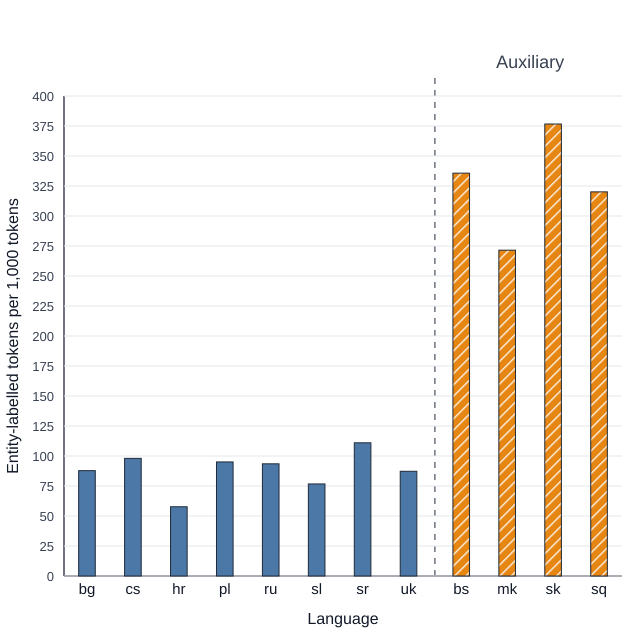
\includegraphics[width=.9\linewidth]{img/entity-density-by-language.png}
  \caption{entity-type distribution per 1{,}000 tokens\newline 
  \hspace*{1.2em}(using only \texttt{LOC}, \texttt{ORG}, and \texttt{PER})}
  \label{fig:entity-density-by-language}
\end{subfigure}%
\begin{subfigure}{.45\textwidth}
  \centering
  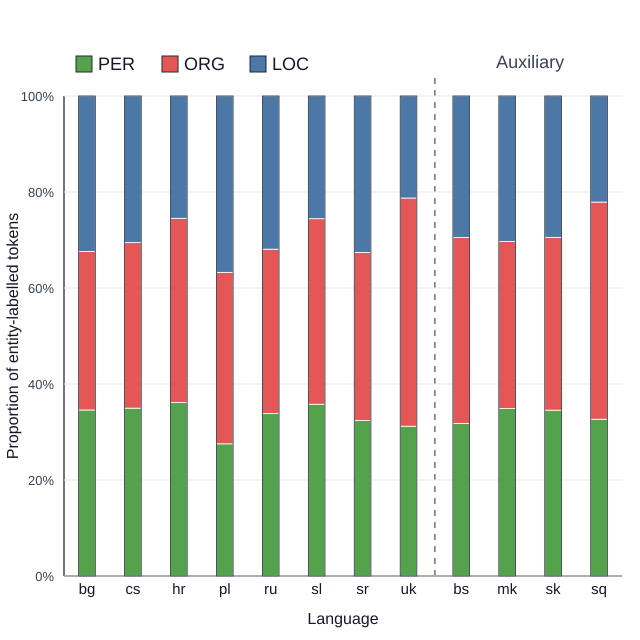
\includegraphics[width=.9\linewidth]{img/label-composition-by-language.png}
  \caption{Normalised label composition by language\newline 
  \hspace*{1.2em}(named entities obtained by collapsing \texttt{B-}\newline
  \hspace*{1.4em} and \texttt{I-} prefixes)}
  \label{fig:label-composition-by-language}
\end{subfigure}
\label{fig:labeldist}
\end{figure}
Even after harmonisation, the corpus collection remains strongly imbalanced in both size and annotation density (see Figure~\ref{fig:entity-density-by-language}). 
When we collapse \texttt{B-} and \texttt{I-} prefixes and consider only \texttt{LOC}, \texttt{ORG}, and \texttt{PER}, the four auxiliary datasets for Bosnian, Macedonian, Slovak, and Albanian contribute 813{,}559 tokens, i.e.\ only 17.8\% of all training tokens, but 278{,}397 entity-labelled tokens, i.e.\ 47.0\% of all \texttt{LOC}/\texttt{ORG}/\texttt{PER} labels. 
By contrast, the eight main language-specific datasets contribute 82.2\% of tokens but only 53.0\% of the collapsed entity labels. 
This difference is reflected in annotation density: the auxiliary group contains 342.2 entity-labelled tokens per 1{,}000 tokens, compared with only 83.7 per 1{,}000 tokens in the main group. 
The auxiliary corpora also have much shorter average sentence length (8.5 vs 20.1 tokens per sentence), which indicates that the multilingual training signal differs not only in corpus provenance but also in segmentation and annotation style.

At the level of label composition, the main and auxiliary groups are surprisingly similar once \texttt{MISC} is removed. 
In the main group, \texttt{LOC}, \texttt{ORG}, and \texttt{PER} account for 28.9\%, 37.4\%, and 33.7\% of all collapsed entity labels, respectively; in the auxiliary group, the corresponding shares are 28.9\%, 37.2\%, and 33.9\%. 
Label composition suggests that the main source of mismatch is not the relative balance between the three shared entity types, but rather the much higher annotation density and shorter sentence segmentation in the auxiliary corpora (see Figure~\ref{fig:label-composition-by-language}). 
For that reason, naive concatenation can overexpose a multilingual model to auxiliary corpora entity supervision. 
We therefore treat the sampling strategy as an explicit experimental factor. 
The balanced multilingual settings equalise language exposure and make cross-language comparisons diagnostic, while the latter full-target and full-pool variants test whether preserving the full target-language evidence changes the practical conclusion.


\section{Methodology}
\label{sec:method}

\subsection{Task setup}
We cast named entity recognition (NER) as token-level sequence labelling on tokenised sentences, using the IOB2 scheme. In the experiments, we predict the three coarse-grained entity types \texttt{LOC}, \texttt{ORG}, and \texttt{PER}, together with the outside label \texttt{O}. 

We consider 12 languages: Bulgarian, Bosnian, Czech, Croatian, Macedonian, Polish, Russian, Slovak, Slovene, Albanian, Serbian, and Ukrainian. We denote the corresponding set of language codes as
\[
L_{12} = \{\texttt{bg}, \texttt{bs}, \texttt{cs}, \texttt{hr}, \texttt{mk}, \texttt{pl}, \texttt{ru}, \texttt{sk}, \texttt{sl}, \texttt{sq}, \texttt{sr}, \texttt{uk}\}.
\]
Following the data-quality distinction introduced in Section~\ref{sec:data}, we define eight main evaluation language datasets and four lower-confidence auxiliary datasets in additional languages:
\[
L_8 = \{\texttt{bg}, \texttt{cs}, \texttt{hr}, \texttt{pl}, \texttt{ru}, \texttt{sl}, \texttt{sr}, \texttt{uk}\}
\text{ and  }
A = \{\texttt{bs}, \texttt{mk}, \texttt{sq}, \texttt{sk}\}.
\]
All main comparisons are reported on $L_8$. The auxiliary group is used only within the multilingual training pool to test whether adding noisier cross-lingual supervision improves or degrades a shared model.

A direct concatenation of all corpora would cause large datasets to dominate multilingual training. 
For each balanced multilingual pool $P$, we therefore define a seed-specific token quota
\[
T_P = \min_{\ell \in P} |D_{\ell}^{\mathrm{train}}|,
\]
where $|D_{\ell}^{\mathrm{train}}|$ is the number of training tokens for language $\ell$ after the 80/10/10 split. 
Therefore, the balanced \texttt{Multi-8} quota is determined by Serbian, the smallest training split in $L_8$, and is approximately $T_{8}=69{,}501$ tokens in the statistics split. 
The balanced \texttt{Multi-12} quota is determined by Albanian, the smallest training split in $L_{12}$, and is approximately $T_{12}=61{,}903$ tokens in the statistics split.

Sampling is performed at the sentence level. 
For each language, we shuffle the training sentences and sample without replacement until the cumulative token count reaches or first exceeds the corresponding quota $T_P$. 
Because complete sentences are retained, the realised token totals can be slightly above the nominal quota. 
Regarding the statistics split, the realised \texttt{Multi-8} language totals range from 69{,}501 to 69{,}540 tokens, while the realised \texttt{Multi-12} totals range from 61{,}903 to 61{,}963 tokens. 
The quota is recomputed separately for each random seed after the seed-specific train--development--test split. 
Within a run, the sampled training pool is fixed and reused across epochs; batches are reshuffled during training, but the multilingual pool is not resampled at every epoch.

This procedure keeps exposure comparable across languages, but it can also heavily downsample large target languages. 
We therefore add full-target and full-pool variants that deliberately relax this balancing constraint to distinguish negative transfer from the loss of target-language evidence.

\subsection{Experimental settings}
We compare six model families.
\begin{enumerate}[leftmargin=*, itemsep=-2pt, topsep=-3pt]
%\begin{itemize}\setlength\itemsep{0.6em}
    \item \textbf{Monolingual baselines (\texttt{Mono-L}).}
    For each evaluation language $L \in L_8$, we train one monolingual model using only the full training set of that language. These runs provide strong practical baselines and reflect the best single-language setting available for each target. Because corpus sizes differ substantially across languages, these baselines are not token-matched across $L$; instead, each language uses all available target-language data.

    \item \textbf{Balanced shared multilingual model on eight languages (\texttt{Multi-8}).}
    We train one shared multilingual model on the eight higher-confidence evaluation languages in $L_8$ using balanced per-language sampling. This condition tests whether a compact shared multilingual model trained on the cleaner subset can match or outperform the corresponding monolingual baselines.

    \item \textbf{Balanced shared multilingual model on twelve languages (\texttt{Multi-12}).}
    We train one shared multilingual model on the full language pool $L_{12} = L_8 \cup A$, again using balanced per-language sampling. 
    This condition tests the balanced twelve-language design: it adds the four lower-confidence auxiliary corpora and, because the quota is recomputed over $L_{12}$, uses a lower per-language quota for the main languages than \texttt{Multi-8}.

    \item \textbf{Target-specific full-target multilingual models (\texttt{Multi8-full-L}).}
    For each target language $L \in L_8$, we train a target-specific multilingual model that retains all available training data for $L$ while adding controlled contributions from the other seven higher-confidence datasets in $L_8 \setminus \{L\}$. This condition asks whether clean multilingual augmentation helps once the target language is no longer downsampled.

    \item \textbf{Leave-one-target-out multilingual pretraining (\texttt{Pretrain-Multi7-full-L}).}
    For each target language $L$, we first train a multilingual model on the seven higher-confidence datasets in $L_8 \setminus \{L\}$, excluding the target language entirely. We then continue fine-tuning on the full target-language training set for $L$. This two-stage setup tests whether the other clean Slavic languages provide a useful pretraining signal before target-only adaptation.

    \item \textbf{Full-pool shared multilingual models.}
    Finally, we train shared multilingual models that preserve all available main-language data rather than balancing each language down to a common quota. \texttt{Full-Multi8} uses the complete $L_8$ pool. \texttt{Full-Multi12} adds all four auxiliary languages. 
    \texttt{Full-Multi12-CapAux} keeps the full $L_8$ pool but caps each auxiliary dataset at $T_{12}$, testing whether lower-confidence WikiANN/PAN-X-derived data are harmful because they are added at all or because they receive too much effective weight.
\end{enumerate}

Together, these settings separate three effects that are otherwise confounded: multilingual transfer, source-data quality, and the amount of target-language evidence retained during training.

\subsection{Target-resource profiles}
To analyse how multilingual gains change as target-language supervision becomes scarcer, we construct target-resource profiles for Serbian (\texttt{sr}) and Slovene (\texttt{sl}). These languages were chosen because they represent opposite ends of the clean-data spectrum in our setup: Serbian is the smallest higher-confidence target language dataset, while Slovene is the largest.

For each target language $g \in \{\texttt{sr}, \texttt{sl}\}$, we define nested training subsets
\[
D_g^{10} \subset D_g^{25} \subset D_g^{50} \subset D_g^{100} = D_g,
\]
corresponding to $10\%$, $25\%$, $50\%$, and $100\%$ of that language's own training data. The percentages are therefore within-language relative budgets rather than matched absolute token counts across languages.

For the monolingual profiles, \texttt{Mono-g@p} is trained only on $D_g^p$, where $p \in \{10,25,50,100\}$. For the multilingual target-specific variants, we reduce only the target-language contribution while keeping the rest of the multilingual pool unchanged. Concretely, in \texttt{Multi-8-g@p} and \texttt{Multi-12-g@p}, the target-language quota is set to
\[
q_g^p = \frac{p}{100}T,
\]
while all non-target languages retain the full multilingual quota $T$.
Here $T$ denotes the quota of the corresponding multilingual pool: $T_8$ for \texttt{Multi-8-g@p} and $T_{12}$ for \texttt{Multi-12-g@p}. 
Consequently, especially for Slovene, monolingual and multilingual results with the same nominal percentage are relative-budget comparisons rather than target-token-matched comparisons.

This design decreases both the amount of unique target-language evidence and its effective weight within the multilingual pool, making the target-resource profiles directly interpretable as a function of target-data scarcity.

\subsection{Model and training configuration}
All experiments use the same pretrained multilingual \texttt{mmBERT-base}~\parencite{marone2025mmbertmodernmultilingualencoder} transformer encoder model and the same optimisation settings; only the composition of the training data changes across runs. 
We use a model from the Hugging Face Transformers library~\parencite{wolf-etal-2020-transformers}, extended with a token classification head.

In the current implementation, we follow the hyperparameter configuration of \textcite{piskorski-etal-2024-cross}, changing only the number of training epochs. 
While their experiments were run for 5 epochs, we trained each model for up to 20 epochs to reduce the risk of underfitting, as low-resource and multilingual NER settings may require more optimisation steps for the model to adapt effectively to sparse target-language evidence.
All remaining settings are kept identical: the maximum sequence length is 256 tokens, the optimiser is AdamW~\parencite{loshchilov2019decoupledweightdecayregularization} with a learning rate of $5 \times 10^{-6}$, and the batch size is 16. 
In total, we evaluate 47 final model configurations, each repeated 3 times with a different random seed that controls the 80/10/10 train--validation--test split, reshuffling, resampling, and model training. 
The \texttt{Pretrain-Multi7-full-L} configurations are two-stage runs, but they are evaluated in the same way as the other final models.

During training, model selection is based on performance on the validation set. For each monolingual baseline, we retain the checkpoint that achieves the highest validation F1-score for its corresponding target language.
For the balanced shared \texttt{Multi-8} and \texttt{Multi-12} models and for the full-pool shared models, checkpoint selection is based on macro-averaged validation-set F1-score across the eight evaluation languages in $L_8$. 
For target-resource profiles and target-specific variants such as \texttt{Multi8-full-sr} or \texttt{Pretrain-Multi7-full-sl}, the final checkpoint is selected based on the validation-set F1-score for the corresponding target language.

\subsection{Evaluation}
We evaluate models using the entity-level micro-averaged F1-score with exact span matching. 
For the main comparison, target-specific recovery experiments, and full-pool shared models, we report per-language F1-scores for all languages in $L_8$, along with the macro-average across these eight languages. 
For the target-resource profiles, we report only the target-language F1-score, since these experiments are designed to measure how multilingual transfer changes as the amount of target-language training data decreases. 
Because the main setup is restricted to \texttt{LOC}, \texttt{ORG}, and \texttt{PER}, all reported scores in the core experiments reflect three-label NER.

In addition to reporting mean F1 over three random seeds, we assess whether model-family differences are consistent across the eight main evaluation languages. 
For each main comparison, we compute paired language-level F1 differences and apply an exact two-sided Wilcoxon signed-rank test over the eight languages. 
We also compute exact sign-test results as a more conservative robustness check. 
Because only three training seeds are available per configuration, we treat seed-level standard deviations as uncertainty estimates rather than as sufficient evidence for per-language significance claims. 
Consequently, statistical tests are used to support corpus-level and model-family conclusions, while individual language differences are interpreted primarily based on effect size and consistency.

\section{Results}
\label{sec:results}

Table~\ref{tab:main_results} reports the mean entity-level F1-score over three random seeds on the eight evaluation languages; standard deviations are shown in the table. Since token-level accuracy is near the ceiling across all settings, we focus primarily on the F1-score.
\begin{table}[H]
\centering
\caption{Main balanced-training results on the eight evaluation languages. Scores are mean entity-level F1 over three seeds, with standard deviations shown after $\pm$. Best scores are boldfaced. Macro F1 is averaged over languages.}
\resizebox{0.91\textwidth}{!}{
\setlength{\tabcolsep}{6pt}
\begin{tabular}{lccccc}
\toprule
Language & Mono & Multi-8 & Multi-12 & $\Delta$(Multi-8$-$Mono) & $\Delta$(Multi-12$-$Multi-8) \\
\midrule
bg    & \textbf{98.51} {\scriptsize$\pm$ 0.10} & 93.12 {\scriptsize$\pm$ 0.26} & 92.87 {\scriptsize$\pm$ 0.06} & -5.39 & -0.26 \\
cs    & \textbf{96.79} {\scriptsize$\pm$ 2.60} & 90.85 {\scriptsize$\pm$ 0.95} & 89.97 {\scriptsize$\pm$ 0.70} & -5.94 & -0.89 \\
hr    & \textbf{96.03} {\scriptsize$\pm$ 3.04} & 90.51 {\scriptsize$\pm$ 0.57} & 89.51 {\scriptsize$\pm$ 0.50} & -5.52 & -1.00 \\
pl    & \textbf{99.04} {\scriptsize$\pm$ 0.04} & 95.37 {\scriptsize$\pm$ 0.07} & 95.16 {\scriptsize$\pm$ 0.34} & -3.68 & -0.21 \\
ru    & \textbf{97.42} {\scriptsize$\pm$ 0.09} & 89.79 {\scriptsize$\pm$ 0.55} & 89.24 {\scriptsize$\pm$ 0.40} & -7.63 & -0.55 \\
sl    & \textbf{97.62} {\scriptsize$\pm$ 1.65} & 90.49 {\scriptsize$\pm$ 0.18} & 89.94 {\scriptsize$\pm$ 0.34} & -7.13 & -0.56 \\
sr    & 97.43 {\scriptsize$\pm$ 2.45} & \textbf{98.38} {\scriptsize$\pm$ 1.25} & 97.65 {\scriptsize$\pm$ 1.77} & +0.96 & -0.74 \\
uk    & \textbf{98.51} {\scriptsize$\pm$ 0.27} & 91.58 {\scriptsize$\pm$ 0.17} & 91.44 {\scriptsize$\pm$ 0.07} & -6.93 & -0.14 \\
\midrule
Macro F1 & \textbf{97.67} & 92.51 {\scriptsize$\pm$ 0.40} & 91.97 {\scriptsize$\pm$ 0.41} & -5.16 & -0.54 \\
\bottomrule
\end{tabular}
}
\label{tab:main_results}
\end{table}

Regarding RQ1, full-data monolingual baselines remain strongest overall. The macro-average F1-score is 97.67 for the monolingual systems, compared with 92.51 for \texttt{Multi-8}, a gap of 5.16 F1-score points. Monolingual training outperforms the shared multilingual model on 7 of the 8 evaluation languages. The only exception is Serbian, where \texttt{Multi-8} improves from 97.43 to 98.38 F1-score (+0.96). The largest multilingual losses are observed for Russian (-7.63), Slovene (-7.13), and Ukrainian (-6.93). In this balanced regime, a single shared multilingual model does not replace strong monolingual baselines, although it can still benefit a smaller target such as Serbian.

Regarding RQ2, adding the four lower-confidence auxiliary datasets does not improve the balanced multilingual model. \texttt{Multi-12} reaches 91.97 macro F1-score, which is 0.54 points below \texttt{Multi-8}. This degradation is consistent across all eight evaluation languages. The largest drops are observed for Croatian (-1.00), Czech (-0.89), Serbian (-0.74), and Slovene (-0.56). 
%These results suggest that treating lower-confidence auxiliary corpora as equally weighted multilingual supervision introduces negative transfer rather than useful complementary evidence.
In this balanced setup, adding lower-confidence auxiliary corpora degrades performance; this likely reflects a combination of lower clean-language quota, high label density in the auxiliary datasets, and annotation/source mismatch.
\begin{table}[H]
\centering
\caption{Relative-budget profiles for Serbian and Slovene. Monolingual budgets are percentages of the full target-language training set, whereas multilingual budgets are percentages of the balanced multilingual target-language quota $T$; Monolingual and multilingual results with the same nominal percentage are relative-budget comparisons. Scores are mean entity-level F1 over three random seeds, with standard deviations shown after $\pm$. The best system within each language and nominal budget is boldfaced.}
\resizebox{0.85\textwidth}{!}{
\setlength{\tabcolsep}{6pt}
\begin{tabular}{rccc|ccc}
\toprule
\multirow{2}{*}{Budget (\%)} & \multicolumn{3}{c|}{Serbian} & \multicolumn{3}{c}{Slovene} \\
\cmidrule(lr){2-4}\cmidrule(l){5-7}
 & Mono & Multi-8 & Multi-12 & Mono & Multi-8 & Multi-12 \\
\midrule
10  & 80.73 {\scriptsize$\pm$ 1.26} & \textbf{93.92} {\scriptsize$\pm$ 0.25} & 92.93 {\scriptsize$\pm$ 1.20} & \textbf{88.97} {\scriptsize$\pm$ 0.35} & 88.31 {\scriptsize$\pm$ 0.36} & 87.62 {\scriptsize$\pm$ 0.51} \\
25  & 91.33 {\scriptsize$\pm$ 1.65} & \textbf{95.33} {\scriptsize$\pm$ 0.71} & 93.89 {\scriptsize$\pm$ 0.95} & \textbf{91.84} {\scriptsize$\pm$ 1.14} & 88.67 {\scriptsize$\pm$ 0.53} & 87.76 {\scriptsize$\pm$ 0.35} \\
50  & 94.58 {\scriptsize$\pm$ 1.24} & \textbf{96.67} {\scriptsize$\pm$ 0.77} & 95.89 {\scriptsize$\pm$ 1.01} & \textbf{94.57} {\scriptsize$\pm$ 1.09} & 89.44 {\scriptsize$\pm$ 0.52} & 88.35 {\scriptsize$\pm$ 0.35} \\
100 & 97.43 {\scriptsize$\pm$ 2.45} & \textbf{98.38} {\scriptsize$\pm$ 1.25} & 97.65 {\scriptsize$\pm$ 1.77} & \textbf{97.62} {\scriptsize$\pm$ 1.65} & 90.49 {\scriptsize$\pm$ 0.18} & 89.94 {\scriptsize$\pm$ 0.34} \\
\bottomrule
\end{tabular}
}
\label{tab:resource_profiles}
\end{table}
Regarding RQ3, the target-resource profiles reveal a strong asymmetry between Serbian and Slovene (Table~\ref{tab:resource_profiles}). 
For Serbian, multilingual training is beneficial across all budgets, with the largest gains in the lowest-resource setting. At 10\% of the Serbian training data, \texttt{Multi-8} exceeds the monolingual baseline by 13.20 F1-score points (93.92 vs 80.73). 
The gain remains positive at 25\% (+4.00), 50\% (+2.09), and even 100\% (+0.96). \texttt{Multi-12} also remains above monolingual performance for Serbian at all budgets, but is consistently below \texttt{Multi-8}. 
In contrast, Slovene remains monolingual-best at every budget. 
The gap between \texttt{Mono-sl} and \texttt{Multi-8} widens as more Slovene training data become available, from +0.66 F1-score at 10\% to +7.13 F1-score at 100\%. 
\texttt{Multi-12} is again consistently below \texttt{Multi-8}.

The first three experiments show that balanced multilingual training is not competitive in aggregate, but they do not by themselves reveal whether this is due to negative multilingual transfer or to the loss of target-language evidence caused by balancing. 

RQ4 addresses this by retaining all target-language data in target-specific multilingual settings.
\begin{table}[h]
\centering
\caption{Target-specific recovery experiments for RQ4. Language-level scores are the mean entity-level F1-score over three random seeds, with standard deviations shown after $\pm$. The best score in each row is boldfaced. Macro F1 is the macro-average of the language-level means; for the shared \texttt{Multi-8} model, the macro-F1 standard deviation over seeds is also reported.}
\resizebox{0.80\textwidth}{!}{
\setlength{\tabcolsep}{6pt}
\begin{tabular}{lcccc}
\toprule
Language & Mono & Multi-8 & Multi8-full-L & Pretrain-Multi7-full-L \\
\midrule
bg & 98.51 {\scriptsize$\pm$ 0.10} & 93.12 {\scriptsize$\pm$ 0.26} & 98.35 {\scriptsize$\pm$ 0.10} & \textbf{98.58} {\scriptsize$\pm$ 0.06} \\
cs & \textbf{96.79} {\scriptsize$\pm$ 2.60} & 90.85 {\scriptsize$\pm$ 0.95} & 96.66 {\scriptsize$\pm$ 2.67} & 96.77 {\scriptsize$\pm$ 2.25} \\
hr & 96.03 {\scriptsize$\pm$ 3.04} & 90.51 {\scriptsize$\pm$ 0.57} & 96.30 {\scriptsize$\pm$ 2.99} & \textbf{96.33} {\scriptsize$\pm$ 2.96} \\
pl & 99.04 {\scriptsize$\pm$ 0.04} & 95.37 {\scriptsize$\pm$ 0.07} & \textbf{99.09} {\scriptsize$\pm$ 0.15} & 99.05 {\scriptsize$\pm$ 0.15} \\
ru & 97.42 {\scriptsize$\pm$ 0.09} & 89.79 {\scriptsize$\pm$ 0.55} & \textbf{97.58} {\scriptsize$\pm$ 0.21} & 96.27 {\scriptsize$\pm$ 1.96} \\
sl & \textbf{97.62} {\scriptsize$\pm$ 1.65} & 90.49 {\scriptsize$\pm$ 0.18} & 97.58 {\scriptsize$\pm$ 1.60} & 97.53 {\scriptsize$\pm$ 1.54} \\
sr & 97.43 {\scriptsize$\pm$ 2.45} & \textbf{98.38} {\scriptsize$\pm$ 1.25} & 98.36 {\scriptsize$\pm$ 1.65} & 98.23 {\scriptsize$\pm$ 1.38} \\
uk & \textbf{98.51} {\scriptsize$\pm$ 0.27} & 91.58 {\scriptsize$\pm$ 0.17} & 98.50 {\scriptsize$\pm$ 0.14} & 98.45 {\scriptsize$\pm$ 0.17} \\
\midrule
Macro F1 & 97.67 & 92.51 {\scriptsize$\pm$ 0.40} & \textbf{97.80} & 97.65 \\
\bottomrule
\end{tabular}
}
\label{tab:target_specific_results}
\end{table}

Table~\ref{tab:target_specific_results} shows that retaining full target-language evidence almost completely recovers the balanced multilingual deficit. \texttt{Multi8-full-L} improves over \texttt{Multi-8} on 7 of 8 languages, with a macro-average of 97.80 compared with 92.51 for \texttt{Multi-8} and 97.67 for \texttt{Mono-L}. 
This confirms that the poor aggregate performance of \texttt{Multi-8} is largely due to target downsampling rather than evidence that clean multilingual training is inherently harmful. \texttt{Multi8-full-L} exceeds the monolingual baseline for Croatian, Polish, Russian, and Serbian, while remaining very close for Bulgarian, Czech, Slovene, and Ukrainian.

The leave-one-target-out pretraining recipe is more mixed. \texttt{Pretrain-Multi7-full-L} reaches 97.65 macro F1, essentially matching the monolingual macro-average but not surpassing \texttt{Multi8-full-L}. 
It gives its clearest improvements for Croatian and Serbian, but it is weaker for Russian and slightly below monolingual performance for Czech, Slovene, and Ukrainian. 
This suggests that other Slavic languages can provide a useful pretraining signal in certain cases, but multilingual pretraining followed by target-only adaptation is not uniformly better than joint full-target multilingual training.

The full-target experiments clarify the source of the balanced Multi-8 loss. 
Multi8-full-L outperforms the shared balanced Multi-8 model across seven of the eight languages, and the language-level Wilcoxon test is significant ($p=0.016$). 
However, Multi8-full-L does not significantly outperform Mono-L overall ($p=0.547$), and Pretrain-Multi7-full-L is also not significantly better than Mono-L ($p=1.000$). 
Therefore, full-target multilingual training primarily recovers the loss due to downsampling, rather than providing a robust overall gain over strong monolingual baselines.

RQ5 shifts from target-specific recipes to the practical question of whether a single shared model can be made competitive by retaining the full main-language pool.

\begin{table}[H]
\centering
\caption{Full-pool shared multilingual variants for RQ5. Scores are mean entity-level F1 over three seeds, with standard deviations shown after $\pm$. The table includes \texttt{Mono-L} and balanced \texttt{Multi-8} for comparison. Best scores are boldfaced.}
\resizebox{0.90\textwidth}{!}{
\setlength{\tabcolsep}{5pt}
\begin{tabular}{lccccc}
\toprule
Language & Mono & Multi-8 & Full-Multi8 & Full-Multi12 & Full-Multi12-CapAux \\
\midrule
bg & 98.51 {\scriptsize$\pm$ 0.10} & 93.12 {\scriptsize$\pm$ 0.26} & 98.63 {\scriptsize$\pm$ 0.08} & \textbf{98.70} {\scriptsize$\pm$ 0.01} & 98.54 {\scriptsize$\pm$ 0.13} \\
cs & \textbf{96.79} {\scriptsize$\pm$ 2.60} & 90.85 {\scriptsize$\pm$ 0.95} & 96.65 {\scriptsize$\pm$ 2.58} & 96.76 {\scriptsize$\pm$ 2.52} & 96.62 {\scriptsize$\pm$ 2.37} \\
hr & 96.03 {\scriptsize$\pm$ 3.04} & 90.51 {\scriptsize$\pm$ 0.57} & \textbf{96.72} {\scriptsize$\pm$ 2.57} & 96.37 {\scriptsize$\pm$ 2.80} & 96.40 {\scriptsize$\pm$ 2.66} \\
pl & 99.04 {\scriptsize$\pm$ 0.04} & 95.37 {\scriptsize$\pm$ 0.07} & 99.06 {\scriptsize$\pm$ 0.04} & \textbf{99.16} {\scriptsize$\pm$ 0.10} & 99.08 {\scriptsize$\pm$ 0.14} \\
ru & 97.42 {\scriptsize$\pm$ 0.09} & 89.79 {\scriptsize$\pm$ 0.55} & 97.54 {\scriptsize$\pm$ 0.10} & \textbf{97.64} {\scriptsize$\pm$ 0.09} & 97.53 {\scriptsize$\pm$ 0.06} \\
sl & \textbf{97.62} {\scriptsize$\pm$ 1.65} & 90.49 {\scriptsize$\pm$ 0.18} & 97.55 {\scriptsize$\pm$ 1.70} & 97.56 {\scriptsize$\pm$ 1.55} & 97.60 {\scriptsize$\pm$ 1.64} \\
sr & 97.43 {\scriptsize$\pm$ 2.45} & 98.38 {\scriptsize$\pm$ 1.25} & 98.51 {\scriptsize$\pm$ 1.31} & \textbf{98.67} {\scriptsize$\pm$ 1.26} & 98.46 {\scriptsize$\pm$ 1.41} \\
uk & 98.51 {\scriptsize$\pm$ 0.27} & 91.58 {\scriptsize$\pm$ 0.17} & 98.62 {\scriptsize$\pm$ 0.16} & 98.49 {\scriptsize$\pm$ 0.31} & \textbf{98.63} {\scriptsize$\pm$ 0.38} \\
\midrule
Macro F1 & 97.67 & 92.51 {\scriptsize$\pm$ 0.40} & 97.91 {\scriptsize$\pm$ 1.02} & \textbf{97.92} {\scriptsize$\pm$ 1.03} & 97.86 {\scriptsize$\pm$ 0.94} \\
\bottomrule
\end{tabular}
}
\label{tab:full_pool_results}
\end{table}

The full-pool shared models substantially alter the practical interpretation (see Table~\ref{tab:full_pool_results}). 
When all main-language training evidence is retained, shared multilingual training becomes competitive with monolingual specialisation: \texttt{Full-Multi8} reaches 97.91 macro F1 and \texttt{Full-Multi12} reaches 97.92, compared with 92.51 for the balanced \texttt{Multi-8} model and 97.67 for the monolingual macro-average. 
This suggests that the poor performance of the balanced shared model is not caused by multilinguality alone. 
Rather, it largely reflects the cost of balancing when this procedure removes substantial evidence in the target language.

The role of the lower-confidence auxiliary datasets is more nuanced. 
In the balanced setting, adding the four auxiliary datasets in additional languages hurts all eight evaluation language datasets, indicating that treating these corpora as equally weighted gold supervision introduces negative transfer. 
In the full-pool setting, however, \texttt{Full-Multi12} is only marginally above \texttt{Full-Multi8}, while \texttt{Full-Multi12-CapAux} is slightly below both on average. 
In \texttt{Full-Multi12-CapAux}, the eight main languages are kept at their full training sizes, while each auxiliary language is capped at the same approximately 61.9k-token quota used in the balanced \texttt{Multi-12} setting.
We find no significant difference among the full-pool variants under the language-level tests.
We consequently do not take RQ5 as evidence that lower-confidence auxiliary data are reliably beneficial. 
The safer conclusion is that auxiliary data are harmful under equal, balanced treatment, but become neutral or, at most, mildly useful once the full, higher-confidence main-language evidence is retained.

\section{Discussion: practical guidance}
\label{sec:discussion}

The experiments suggest four practical guidelines for Slavic NER.
First, if the goal is the strongest target-specific system and enough target-language data are available, a monolingual model or a full-target multilingual model should be preferred over a balanced shared model. The comparison between \texttt{Multi-8} and \texttt{Multi8-full-L} shows that balancing can impose a large target-evidence penalty.
Second, if the target language is genuinely low-resource, clean multilingual transfer can be highly valuable: Serbian gains 13.20 F1-score points at the 10\% budget and remains above monolingual training even at 100\%.
Third, lower-confidence auxiliary corpora should not be treated as interchangeable with manually curated data. 
Their high annotation density and short sentence segmentation make them a distinct source of supervision, and equal weighting hurts in the balanced \texttt{Multi-12} setting.
Fourth, if deployment requires a single maintainable model across the main languages, full-pool shared training is more promising than balanced shared training. \texttt{Full-Multi8} and \texttt{Full-Multi12} recover monolingual-level macro performance while preserving the operational advantage of one model.

These guidelines also clarify the role of leave-one-target-out pretraining. \texttt{Pretrain-Multi7-full-L} is scientifically useful because it asks whether other languages help without seeing the target language during multilingual pretraining. 
In practice, however, it is not consistently better than either monolingual training or joint full-target multilingual training. 
It should therefore be viewed as an optional transfer recipe for selected low-resource targets, not as the default choice.

Taken together, the results indicate that multilingual Slavic NER performance is influenced less by the sheer number of languages included than by the source quality, target-language evidence, and the chosen sampling strategy.
Balanced multilingual training is useful for diagnostics. 
It can strongly help a small target such as Serbian, but full-target or full-pool training is the better recipe when sufficient target-language data are available.

This study has several limitations that qualify the interpretation of the results. 
First, all experiments use a single multilingual encoder, \textsc{mmBERT}, so the observed effects may depend on this particular model family and may differ for newer or larger multilingual encoders.
Second, the analysis is based on aggregate entity-level F1 scores and does not break down performance by entity type, entity length, frequency, or ambiguity. 
Third, the evaluation uses random splits, which are appropriate for controlled comparisons between training regimes, but they do not test robustness to document-level, temporal, topical, or cross-corpus shifts. 

\section{Conclusion}
\label{sec:conclusion}

We presented a multilingual NER study for Slavic languages covering 12 training languages and 8 main evaluation languages, with all corpora harmonised to a shared three-label \texttt{LOC}/\texttt{ORG}/\texttt{PER} setup. 
The central result is that multilingual transfer is not a single yes-or-no decision. 
Its value depends on the target-resource size, the source-data quality, and whether the training recipe preserves sufficient target-language evidence.

In the balanced shared setting, a single \texttt{Multi-8} model did not replace strong monolingual baselines; it achieved 92.51 macro F1, compared with 97.67 for \texttt{Mono-L}. 
The exception was Serbian, where multilingual training outperformed monolingual training, and the target-resource profiles showed particularly large gains at low data budgets. 
Adding four lower-confidence auxiliary datasets in the balanced \texttt{Multi-12} setting consistently reduced performance, confirming that more languages are not inherently better when their annotation styles and corpus properties differ from those of the main evaluation data.

The additional full-target and full-pool experiments refine this conclusion. 
When all target-language data are retained, \texttt{Multi8-full-L} recovers most of the balanced model's deficit and slightly exceeds the monolingual macro-average. 
Likewise, shared \texttt{Full-Multi8} and \texttt{Full-Multi12} models reach about 97.9 macro F1, showing that a single multilingual model can be practically competitive when it does not discard high-confidence target evidence. 
Leave-one-target-out pretraining is useful in certain cases, but it is not uniformly stronger than joint full-target multilingual training.

For practitioners, the resulting guidance is straightforward. Use clean multilingual transfer for genuinely low-resource targets; avoid giving lower-confidence auxiliary corpora the same status as manually curated data; and, when a shared model is needed, preserve full main-language evidence rather than enforcing strict balance. In this sense, the main lesson is quality over quantity, but also target evidence over artificial balance.

\section{Reproducibility and availability}

The experiments are reproducible with the code available at \url{https://github.com/ivlcic/cannopy}. 
In addition, the multilingual variant of the \texttt{Full-Multi12} model is available on Hugging Face \url{https://huggingface.co/ivlcic/sour-sarma}.

\acknowledgmenteng{This work was funded by the Slovenian Research and Innovation Agency (ARIS) through the core research programme P2-0103 (Knowledge Technologies) and the project L2-50070 (Embeddings-based techniques for Media Monitoring Applications). The work of J.C. was supported by the Young Researcher Grant PR-13409.}

\urlstyle{same} 
\printbibliography

\newpage
\titleeng{Kdaj je večjezični prenos koristen za prepoznavanje imenskih entitet v slovanskih jezikih?}
\begin{abstracteng}
V prispevku preučujemo, kdaj je večjezični prenos v praksi koristen za prepoznavanje imenskih entitet v slovanskih jezikih (NER).
Heterogenim korpusom dvanajstih jezikov uskladimo označevalno shemo IOB2 s tremi skupnimi tipi entitet: LOC, ORG in PER.
Poskuse smo izvedli na ročno označenih podatkovnih zbirkah osmih jezikov, ter na pomožnih samodejno zgrajenih korpusih z nižjo stopnjo zaupanja za dodatne štiri jezike.
Analiziramo vplive večjezičnega združevanja, kakovosti podatkov (ročno označene v primerjavi s samodejno zgrajenimi podatkovnimi zbirkami), obsega virov za ciljni jezik in ohranjanja učinkov ciljnega jezika.
Sprašujemo se, ali lahko uravnotežen skupni večjezični model nadomesti močne enojezične izhodiščne modele, ali pomožni korpusi z nižjo stopnjo zaupanja pomagajo ali škodujejo, kako se prenos spreminja ob zmanjšani količini učnih podatkov za ciljni jezik in ali lahko večjezično učenje z vsemi podatki ciljnega jezika, oziroma z vsemi podatki v združenem naboru, zmanjša razliko v primerjavi z enojezičnimi modeli.
Rezultati kažejo, da uravnoteženo večjezično učenje ni univerzalna zamenjava za enojezično specializacijo, lahko pa izrazito koristi ciljnim jezikom z manj viri.
Dodajanje pomožnih korpusov z nižjo stopnjo zaupanja pri učenju kot enakovredne povzroča negativni prenos, medtem ko ohranjanje vseh podatkov ciljnega jezika veča konkurenčnost večjezičnih modelov.
Na splošno je večjezični prenos za prepoznavanje imenskih entitet v slovanskih jezikih koristen le, kadar so kakovost izvornih podatkov, obseg virov za ciljni jezik in strategija vzorčenja, skrbno nadzorovani.
Nastali večjezični model za prepoznavanje imenskih entitet javno objavljamo na platformi Hugging Face: \url{https://huggingface.co/ivlcic/sour-sarma}.
\end{abstracteng}

\keywordsslo{večjezično prepoznavanje imenskih entitet, medjezikovni prenos, slovanski jeziki, obdelava naravnega jezika pri omejenih virih, večjezična obdelava naravnega jezika}

\end{document}